\documentclass{ieeetj}
\usepackage{cite}
\usepackage{amsmath,amssymb,amsfonts}
\usepackage{algorithmic}
\usepackage{graphicx,color}
\usepackage{textcomp}
\usepackage{xcolor}
\usepackage{hyperref}
\usepackage{orcidlink}
%\hypersetup{hidelinks=true}
\usepackage{algorithm,algorithmic}
\def\BibTeX{{\rm B\kern-.05em{\sc i\kern-.025em b}\kern-.08em
    T\kern-.1667em\lower.7ex\hbox{E}\kern-.125emX}}
\newcommand{\encS}[1]{E_{\mathrm{slot}}\!\left(#1\right)}
\newcommand{\decS}[1]{D_{\mathrm{slot}}\!\left(#1\right)}
\newcommand{\dslots}{\mathbf{d}_{\mathrm{slots}}}
\AtBeginDocument{\definecolor{tmlcncolor}{cmyk}{0.93,0.59,0.15,0.02}\definecolor{NavyBlue}{RGB}{0,86,125}}



\def\OJlogo{\vspace{-4pt}$<$Society logo(s) and publication title will appear here.$>$}
\def\seclogo{\vspace{10pt}$<$Society logo(s) and publication title will appear here.$>$}

\def\authorrefmark#1{\ensuremath{^{\textbf{#1}}}}

\begin{document}
\receiveddate{XX Month, XXXX}
\reviseddate{XX Month, XXXX}
\accepteddate{XX Month, XXXX}
\publisheddate{XX Month, XXXX}
\currentdate{XX Month, XXXX}
\doiinfo{XXXX.2022.1234567}

\markboth{BRINGING PRIVATE READS TO HYPERLEDGER FABRIC VIA PRIVATE INFORMATION RETRIEVAL }
{IASENOVETS ET AL.}

\title{Bringing Private Reads to Hyperledger Fabric via Private Information Retrieval}

\author{ARTUR IASENOVETS~\orcidlink{0009-0008-0008-3746}\authorrefmark{1},
FEI TANG~\orcidlink{0000-0002-0048-9876}\authorrefmark{1},
HUIHUI ZHU~\orcidlink{0009-0006-5701-1837}\authorrefmark{2},
PING WANG~\orcidlink{0009-0003-3832-2494}\authorrefmark{2} and
LEI LIU~\orcidlink{0009-0001-3851-4854}\authorrefmark{2}}
\affil{School of Cybersecurity and Information Law, Chongqing University of Posts and Telecommunications, Chongqing 400065, China}
\affil{School of Computer Science and Technology, Chongqing University of Posts and Telecommunications, Chongqing 400065, China}
\corresp{CORESSPONDING AUTHOR: FEI TANG (email: tangfei@cqupt.edu.cn).}
\authornote{This work was supported in part by the National Key Research and Development Program of 
China under Grant 2021YFF0704102, in part by the Key Project of Science and Technology Research by Chongqing Education Commission under 
Grant KJZD-K202400610, and in part by the Chongqing Natural Science Foundation General Project under Grant CSTB2025NSCQ-GPX1263.}

\begin{abstract}
    Permissioned blockchains ensure integrity and auditability of shared data but expose 
    query parameters to peers during read operations, creating privacy risks for organizations querying sensitive records. 
    This paper proposes a Private Information Retrieval (PIR) mechanism to enable \emph{private reads} from Hyperledger Fabric’s 
    world state, allowing endorsing peers to process encrypted queries without learning which record is accessed. We implement and benchmark a PIR-enabled 
    chaincode that performs ciphertext–plaintext (\emph{ct×pt}) homomorphic multiplication directly within \emph{evaluate} 
    transactions, preserving Fabric’s endorsement and audit semantics. The prototype achieves an average end-to-end latency 
    of 113~ms and a peer-side execution time below 42~ms, with approximately 2~MB of peer network traffic per private read in 
    development mode—reducible by half under in-process deployment. Storage profiling across three channel configurations shows 
    near-linear growth: block size increases from 77 kilobytes to 294 kilobytes and world-state from 112 kilobytes to 
    332 kilobytes as the ring dimension scales from 8,192 to 32,768 coefficients. Parameter analysis further indicates that 
    ring size and record length jointly constrain packing capacity, supporting up to 512~records of 64~bytes each 
    under the largest configuration. These results confirm the practicality of PIR-based \emph{private reads} in Fabric 
    for smaller, sensitive datasets and highlight future directions to optimize performance and scalability.
  \end{abstract}
    
\begin{IEEEkeywords}
    Private Information Retrieval (PIR), Hyperledger Fabric, Private Reads, Query Privacy.
\end{IEEEkeywords}

%\IEEEspecialpapernotice{(Invited Paper)}

\maketitle
\section{INTRODUCTION}\label{sec:introduction}

\subsection{MOTIVATION AND PROBLEM STATEMENT}
Blockchain \cite{nakamoto_bitcoin_2008} is a peer-to-peer network protocol that uses cryptographic primitives and 
a consensus mechanism to create and maintain a distributed ledger of transactions, such as those in Ethereum \cite{wood_ethereum_2014} and 
Hyperledger Fabric \cite{androulaki_hyperledger_2018}.

Hyperledger Fabric (HLF or Fabric) is widely adopted in various domains, one of them being Cyber Threat Intelligence (CTI) sharing
\cite{dunnett_trusted_2022, huff_distributed_2021, allouche_trade_2021, gong_blocis_2020}, where multiple organizations 
exchange threat indicators and wish to keep their queries confidential not to be associated with specific threats or incidents.
Blockchain guarantees, however, primarily cover data integrity and auditability, not query privacy.
This issue was recently highlighted by Ethereum's privacy special interest group in their
``PSE Roadmap: 2025 and Beyond''~\cite{ethereum_pse_2025}, where they also 
emphasized the need for \emph{private reads} next to private writes and private voting.

In Hyperledger Fabric~\cite{androulaki_hyperledger_2018}, the separation of \emph{evaluate} and \emph{submit} 
makes the read-privacy gap explicit: an \emph{evaluate} call is a read-only proposal sent to endorsing peers, 
which execute the chaincode and return results without committing to the ledger \cite{fabric_docs_a_nodate}.
Crucially, these peers still observe all function arguments and read-sets, creating a privacy risk if queries are sensitive.

This motivates us to target the \emph{read} privacy issue in Fabric, defined as the ability to 
hide which record is being queried from endorsing peers during \emph{evaluate}-type calls. 
Given the problem description, an obvious approach is to construct and use a Private Information Retrieval (PIR)~\cite{chor_private_1998} 
protocol, which would enable a client to retrieve an item from a world state database without revealing to the peer which item was requested. 
However, integrating PIR into Fabric's architecture presents unique challenges, as discussed next.

\subsection{PIR SCHEME SELECTION}
Private Information Retrieval (PIR) spans \emph{information-theoretic} (IT-PIR) and \emph{computational} (CPIR) designs, 
and each can be either \emph{non-preprocessing} or \emph{preprocessing}~\cite{chor_private_1998}. IT-PIR achieves unconditional 
privacy with multiple non-colluding servers~\cite{goldberg_improving_2007,beimel_breaking_2002,devet_optimally_2012,demmler_raid-pir_2014}, 
which is hard to guarantee in consortium ledgers. Single-server CPIR without preprocessing (e.g., SealPIR, FastPIR, OnionPIR, 
Spiral~\cite{sealpir_2018,fastpir_2021,onionpir_2021,spiral_2022}) uses homomorphic encryption and fits Fabric’s one-round \emph{evaluate} 
path, avoiding per-client state but incurring higher computational costs. Preprocessing CPIR (SimplePIR, Piano, HintlessPIR, YPIR; and other 
doubly-efficient variants~\cite{beimel_reducing_2004,simplepir_2023,piano_pir_2024,hintless_pir_2024,ypir_2024,depir_ring_lwe_2023,okada_towards_depir_2025,corrigan-gibbs_subpir_2020}) 
reduces online cost via client/server ``hints,'' yet in Fabric this implies large client downloads or per-client peer state, conflicting 
with stateless, deterministic transactions. Consequently, we adopt the standard design pattern of single-server, HE-based, 
non-preprocessing CPIR construction for \emph{private reads}, while \emph{not claiming to instantiate} any existing PIR scheme verbatim. 
This preserves Fabric’s endorsement semantics, avoids hint management, and aligns with a single query–response 
interaction. While compute- and packing-limited, this choice is practical for smaller, sensitive datasets in permissioned settings, 
as our evaluation shows in~\ref{sec:evaluation}.

\subsection{RELATED WORK}
We now review prior efforts to integrate PIR with blockchain and distributed systems to enhance query privacy. 
A detailed comparison is provided in Table~\ref{tab:comparison-related} in Section~\ref{sec:discussion}.

Xiao et al.~\cite{xiao_cloak_2024} propose Cloak, a privacy-preserving blockchain query scheme that uses distributed point functions (DPF) 
and noise-based sub-requests to hide the retrieval information, achieving communication costs of 0.2-0.5 KB and query latency of 0.4-0.5 ms 
for databases with 4-64 records of 16-32 bytes each.

Mazmudar et al.~\cite{mazmudar_peer2pir_2025} propose Peer2PIR, a privacy solution for IPFS using a combination of PAILLIERPIR and RLWEPIR schemes 
to hide query content across peer routing, provider advertisements, and content retrieval functionalities.
For the relevant private content retrieval function, they achieve communication costs of 10-15~MB and latencies of 0.5-15~s for 
databases of 1,000 to 1,000,000 records with 256~KB content blocks using the Spiral~\cite{spiral_2022} protocol.

Kaihua et al.~\cite{Kaihua2019applying} design an SPV protocol for lightweight Bitcoin clients using a hybrid PIR scheme (combining IT-PIR and C-PIR)
to enhance query privacy over Bloom-filter-based methods. For a single transaction verification in the weekly database, it achieves a 
communication cost of 666~KB and latency of 2.84~s for databases with 7,688-512,460 records of 62-876 bytes each.

Kumar et al. introduced a series of HLF frameworks that integrate Private Information Retrieval (PIR) across different domains, 
namely BRON~\cite{kumar_bron_2024} and DEBPIR~\cite{kumar_debpir_2025}. Although posed as enabling PIR functionality,
their evaluations primarily focus on the system's write throughput rather than the specific performance of PIR queries.

\textbf{Targeted gap.}
Permissioned ledgers like Hyperledger Fabric ensure integrity and auditability of shared data but leak function arguments and read-sets
to endorsing peers during \emph{evaluate} calls, creating privacy risks in multi-organisation settings.
While prior works have explored PIR integration in various blockchain and distributed systems contexts,
none have specifically addressed the challenge of enabling \emph{private reads} in Hyperledger Fabric without modifying its core architecture.
To fill this gap, we explore how to enable \emph{private reads} from Fabric’s world state by integrating a HE-based PIR mechanism directly into chaincode, 
and we evaluate its practicality through detailed benchmarks and parameter studies.

\subsection{KEY OBJECTIVE AND CONTRIBUTIONS}
In this work, we demonstrate that HE-based PIR can be implemented natively in chaincode to enable \emph{private reads} in 
Hyperledger Fabric under \emph{evaluate} calls and achieve practical performance under certain parametrization choices.

Hence, the main contributions of this work are:
\begin{enumerate}
    \item \textbf{Enabling Private Reads in Hyperledger Fabric.} 
    We introduce the first end-to-end design, implementation and evaluation of a private information retrieval (PIR) mechanism, 
    leveraging homomorphic encryption, natively integrated into Hyperledger Fabric chaincode. This enables clients to perform \emph{private read} 
    operations on the world state through \emph{evaluate} transactions, ensuring the queried key remains confidential from endorsing peers.
    Our approach requires no modifications to Fabric’s core, demonstrating a practical, \emph{plug-in privacy layer} for state queries.
    \item \textbf{Polynomial database construction.}
    We formalize the mapping between Fabric’s key–value world state and a homomorphically encodable polynomial database, 
    deriving feasibility constraints that link record length, ring dimension, and slot allocation. 
    These relationships ensure the correctness of homomorphic retrieval and guide practical parameter selection for real-world datasets.
    \item \textbf{Multi-channel approach.} 
    To overcome database size limits imposed by polynomial packing constraints, we propose a multi-channel architecture 
    where each channel hosts a specific HE parameter set and corresponding polynomial database instance, 
    enabling clients to select appropriate channels based on their query needs.
    \item \textbf{Comprehensive evaluation.} 
    We implement a prototype using the Lattigo~\cite{noauthor_lattigo_2024} library and benchmark the cryptographic operations, 
    blockchain interactions, and end-to-end query latency under various configurations. Our results show that single-query latencies 
    remain practical for typical Fabric deployments.
    \item \textbf{Open-Source Release.} To encourage reproducibility, we release the full implementation of our Fabric 
    chaincode, client logic and benchmarks at the repository: \url{https://github.com/iasenovets/2_2_HLF_CPIR}.
\end{enumerate}

\subsection{ORGANIZATION}

The remainder of this paper is organized as follows: 
Section~\ref{sec:preliminaries} reviews Fabric's privacy features, database limits, homomorphic encryption-based PIR, and notation.
Section~\ref{sec:proposed_system} describes our system and threat models, polynomial database construction, feasibility constraints, 
multi-channel architecture, workflow and algorithms.
Section~\ref{sec:security} analyzes security.
Section~\ref{sec:evaluation} shows experimental setup, cryptographic and blockchain benchmarks, and overall system performance.
Section~\ref{sec:discussion} discusses limitations and future directions, and Section~\ref{sec:conclusion} concludes the paper.

\section{PRELIMINARIES}\label{sec:preliminaries}

\subsection{FABRIC NATIVE PRIVACY FEATURES}
We hereby acknowledge several native solutions for privacy that Hyperledger Fabric provides and explain why they do not fully address the 
query privacy problem.

\textbf{Separate Channels.} Fabric's multi-channel architecture~\cite{fabric_docs_a_nodate} isolates ledgers across subgroups of organizations, 
limiting which participants observe which data. 
However, channel separation controls \emph{who} sees a ledger, query intent remains visible to all endorsers of a channel.

\textbf{Private Data Collections (PDC).} PDCs~\cite{fabric_docs_a_nodate} restrict which organizations store and access private key–value pairs. 
The shared ledger records only hashes, while members of the collection hold plaintext. 
PDCs provide access control but still expose function arguments to endorsers inside the collection, leaving query patterns observable.

\textbf{Fabric Private Chaincode (FPC).} FPC~\cite{fabric_docs_a_nodate, brandenburger_blockchain_2018} executes chaincode within Intel SGX enclaves. 
Arguments and state are protected even from peer operators, but this requires Trusted Execution Environments (TEEs) and attestation, 
introducing additional hardware and trust assumptions.

\subsection{FABRIC STORAGE LIMITS}
We here address the question of how large a database can be stored in Fabric world state and ledger history, as this impacts the 
practical limits of our PIR construction.

\textbf{World state (LevelDB/CouchDB).}
Fabric imposes no hard limit on the number of key–value entries in world state; capacity depends on available disk space and peer I/O throughput.
In our implementation, each channel maintains a few small artifacts in world state that amount up to a 350~KB under typical parameters (see Section~\ref{sec:evaluation}), 
LevelDB is sufficient and preferable for performance and simplicity, while CouchDB~\cite{fabric_docs_a_nodate} remains an option to extend from 8~MB to 4~GB if needed.

\textbf{Ledger history (blockchain log).}
According to the documentation~\cite{fabric_docs_a_nodate}, block size is constrained by the ordering service configuration. 
By default, the Fabric orderer limits the serialized payload to \emph{AbsoluteMaxBytes~=~10~MB} (recommended under 49~MB given the gRPC ceiling of 100~MB), 
and typically aggregates up to \emph{MaxMessageCount~=~500} transactions per block or \emph{PreferredMaxBytes~=~2~MB}.
In our system, these limits affect only \emph{submit} transactions such as \texttt{InitLedger} or record updates. 
\emph{Evaluate} transactions (including \texttt{PIRQuery}) are read-only and do not generate blocks, thus unaffected by ordering or batching constraints.

\textbf{Implication.}
The effective capacity of a channel is governed primarily by cryptographic feasibility defined in Section~\ref{sec:proposed_system},
and the size of a single world-state value (i.e., \emph{$m_{DB}$}), rather than by Fabric’s block or database limits. 
For very large objects, an optional extension is to store them off-chain 
in IPFS~\cite{benet_ipfs_2014} while persisting only their content identifiers (CIDs) in world state, 
keeping the polynomial \emph{$m_{DB}$} as the structured component used for private retrieval.

\subsection{HE-BASED PIR}
\textbf{Homomorphic Encryption.}
Lattice-based homomorphic encryption schemes, such as Brakerski/ Fan-Vercauteren (BFV), Brakerski-Gentry-Vaikuntanathan 
(BGV), CKKS and TFHE~\cite{cryptoeprint:2012/144,cryptoeprint:2011/277,cheon_homomorphic_2017,cryptoeprint:2018/421} have emerged as 
foundational technologies for practical CPIR implementations.

We base our CPIR construction on the BGV scheme, a lattice-based homomorphic encryption based on 
the Ring Learning With Errors (RLWE) problem~\cite{peikert_lattice_2014}, which supports both addition and multiplication over ciphertexts.
The BGV~\cite{cryptoeprint:2011/277} scheme defines operations over two polynomial rings: 
a ciphertext ring $R_Q = \mathbb{Z}_Q[X]/(X^N+1)$ and a plaintext ring $R_T = \mathbb{Z}_T[X]/(X^N+1)$, 
both sharing the same dimension $N=2^{\log N}$. 
In our implementation, these rings are jointly specified by a single parameter literal 
$(\log N, \log Q_i, \log P_i, T)$ as provided by the Lattigo library \cite{noauthor_lattigo_2024} and paper~\cite{mouchet_multiparty_2020}.
The field $T$ determines $R_T$, while the modulus chain $(Q,P)$ and their bit-lengths $(\log Q_i, \log P_i)$ 
determine $R_Q$.

\textbf{CPIR Definition.}
Model the database as $D=\{d_0,\dots,d_{n-1}\}$. At the record level, selecting
$d_i$ can be represented abstractly by a one-hot vector $e_i\in\{0,1\}^{n}$.
In our implementation, however, each serialized record occupies a fixed logical
slot window $J_i=\{i\cdot record_s,\dots,(i+1)\cdot record_s-1\}$.
The client therefore uses the expanded slot selector $v_i\in\{0,1\}^{N}$,
where $v_i[j]=1$ for $j\in J_i$ and $v_i[j]=0$ otherwise. Although $v_i$
contains $record_s$ nonzero entries, it selects one logical record. The client
batch-encodes and encrypts this selector as
$m_q=\encS{v_i}$ and $ct_q=\emph{Enc}_{pk}(m_q)$.

\textbf{CPIR Instantiation.}
We instantiate Computational PIR using the algorithms
$(\emph{KeyGen},\emph{Enc},\emph{Eval},\emph{Dec})$ together with the
batched slot encoder $E_{\mathrm{slot}}$ and decoder $D_{\mathrm{slot}}$:
\begin{itemize}
    \item $\emph{KeyGen}(\lambda)\rightarrow(pk,sk)$: output a public and secret key pair.
    \item $\emph{Enc}_{pk}(\encS{v_i})\rightarrow ct_q$: batch-encode the
    slot-level window selector and encrypt the resulting plaintext.
    \item $\emph{Eval}(ct_q,m_{DB})\rightarrow ct_r$: multiply the query
    ciphertext by the encoded plaintext database $m_{DB}=\encS{\dslots}$.
    \item $\emph{Dec}_{sk}(ct_r)\rightarrow m_r$: decrypt the encrypted response
    to a plaintext, which is then slot-decoded as $u=\decS{m_r}$.
\end{itemize}

\noindent\textbf{Correctness.}
Let $\dslots=\operatorname{SerializePadSlots}(D)\in\mathbb{Z}_T^N$ and
$m_{DB}=\encS{\dslots}$. Correctness requires
\[
\begin{aligned}
ct_r&=\emph{Eval}\!\left(\emph{Enc}_{pk}(\encS{v_i}),m_{DB}\right),\\
u&=\decS{\emph{Dec}_{sk}(ct_r)}=v_i\odot\dslots\pmod T,
\end{aligned}
\]
followed by
\[
d_i=\operatorname{Deserialize}\!\left(
\operatorname{Unpad}\!\left(u[J_i]\right)\right).
\]
Thus $ct_r$ encrypts an $N$-slot masked vector; the client recovers $d_i$ by
decoding and extracting its known window rather than by an inner-product reduction.

\noindent \textit{Remark (restricted operation set).} 
The full BGV scheme also provides $\texttt{EvalKeyGen}$ to generate relinearization and rotation keys,
supporting ciphertext–ciphertext multiplication ($ct \times ct$), automorphisms, and modulus switching.
Since the database \emph{$m_{DB}$} is stored in plaintext within world state,
our PIR construction only requires homomorphic ciphertext–plaintext multiplication ($ct \times pt$).
The single multiplication is sufficient because batched BGV multiplication
decodes to componentwise slot multiplication. It masks nonselected slots but
does not rotate, sum, or move the selected record to a distinguished slot.
Further extension to ciphertext–ciphertext operations is possible but incurs additional overhead, as discussed in Section~\ref{sec:discussion}.

\subsection{NOTATION}
We summarize the main notation used throughout the paper in Table~\ref{tab:notation}.

\begin{table}[!ht]
\caption{Notation}
\label{tab:notation}
\setlength{\tabcolsep}{6pt}
\renewcommand{\arraystretch}{1.1}
    \begin{tabular}{|l|l|}
    \hline
    \textbf{Symbol} & \textbf{Description} \\
    \hline
    $\lambda$ & Security parameter \\
    \hline
    $pp$ & Public parameters (metadata) \\
    \hline
    $n$ & Database size; \\ & index domain $[n]=\{0,\dots,n-1\}$ \\
    \hline
    $D$ & Database records $\{d_0,\dots,d_{n-1}\}$ \\
    \hline
    $e_i$ & Record-level one-hot abstraction for index $i$ \\
    \hline
    $J_i$ & Logical slot window occupied by record $d_i$ \\
    \hline
    $\dslots$ & Serialized and padded database \\ & slot vector in $\mathbb{Z}_T^N$ \\
    \hline
    $v_i$ & Expanded one-hot/windowed slot \\ & selector $\mathbf{1}_{J_i}$ \\
    \hline
    $E_{\mathrm{slot}},D_{\mathrm{slot}}$ & Batched slot encode / decode maps \\
    \hline
    $m_{DB}$ & Encoded database plaintext $\encS{\dslots}$ \\
    \hline
    $m_q$ & Encoded selector plaintext $\encS{v_i}$ \\
    \hline
    $u$ & Decoded masked vector $v_i\odot\dslots$ \\
    \hline
    $\emph{Enc}_{pk}(\cdot)$, $\emph{Dec}_{sk}(\cdot)$ & Encrypt / Decrypt \\
    \hline
    $\emph{Eval}(\cdot)$ & Homomorphic evaluation \\ & (ct–pt multiply) \\
    \hline
    $pk,\, sk$ & Public / secret keys \\
    \hline
    $ct_q$ & Encrypted encoded selector $\emph{Enc}_{pk}(m_q)$ \\
    \hline
    $ct_r$ & Encrypted masked-vector response \\ & $\emph{Eval}(ct_q,m_{DB})$ \\
    \hline
    $d_i$ & Record reconstructed from $u[J_i]$ \\
    \hline
    $\emph{KeyGen}(\lambda)$ & Key generation $\!\to\!(pk,sk)$ \\
    \hline
    $N$ & Ring dimension \\
    \hline
    $\log N$ & Logarithm base 2 of ring \\ & dimension $N$ \\
    \hline
    $\log Q_i$ & Bit-lengths of primes \\ & forming modulus chain $Q$ \\
    \hline
    $\log P_i$ & Bit-lengths of special primes $P$ \\
    \hline
    $T$ & Plaintext modulus \\
    \hline
    $record_s$ & Slots allocated per record \\
    \hline
    $record_b$ & Base serialized size of a record in bytes \\
    \hline
    $record_{\mu,\log N}$ & Template-specific minimum \\
    \hline
    $\mathcal{S}$ & Allowed discrete slot sizes \\
    \hline
    $|\cdot|$, $\mathrm{size}(\cdot)$ & Length in elements / bytes \\
    \hline
    $\mathcal{C}(N,s,n)$ & Capacity predicate: $n \cdot s \leq N$ \\
    \hline
    $\mathcal{M}(\log N,s)$ & Template predicate: $s \geq record_{\mu,\log N}$ \\
    \hline
    $\mathcal{D}(s)$ & Discrete predicate: $s \in \mathcal{S}$ \\
    \hline
    $\mathcal{F}(\log N,s,n)$ & Feasibility tuple: $\mathcal{C} \wedge \mathcal{M} \wedge \mathcal{D}$ \\
    \hline
    $\mathcal{DO},\,\mathcal{DW},\,\mathcal{DR},\,\mathcal{GW}$ & Data Owner; Data Writer; \\ & Data Requester; Gateway \\
    \hline
    \emph{evaluate}, \emph{submit} & Fabric read / write transaction types \\
    \hline
    $\mathcal{L}$ & Leakage considered \\ & (ciphertext size, protocol timing) \\
    \hline
    \end{tabular}
\end{table}
    
\section{PROPOSED SYSTEM}\label{sec:proposed_system}
\subsection{SYSTEM MODEL}
We introduce a blockchain-based query privacy system designed for permissioned ledgers. 
The system enables clients to perform \emph{private reads} from the ledger while endorsing peers can evaluate 
read-only queries over encrypted inputs without learning which record was accessed.  
We achieve this by integrating a lattice-based CPIR scheme based on the
BGV~\cite{cryptoeprint:2011/277} homomorphic encryption scheme directly into Fabric chaincode.
This approach ensures that clients remain the sole holders of decryption keys, while peers perform only 
black-box computations, thereby enhancing overall privacy without requiring trusted hardware or protocol modifications.

\noindent Our system is composed of the following entities:

\begin{itemize}
    \item \textbf{Data Owner ($\mathcal{DO}$):} Endorsing peers that hold the current plaintext 
    polynomial \emph{$m_{DB}$} in world state and execute PIR during \emph{evaluate}. $\mathcal{DO}$ is honest-but-curious.
    \item \textbf{Data Writer ($\mathcal{DW}$):} A client organization that provisions or refreshes 
    the database. $\mathcal{DW}$ invokes \emph{submit} to initialize the ledger (e.g., set $n$ and template bounds). 
    Chaincode computes $record_s$, packs $D=\{d_0,\dots,d_{n-1}\}$, encodes it into \emph{$m_{DB}$}, and persists it.
    \item \textbf{Data Requester ($\mathcal{DR}$):} A client that privately retrieves a record. $\mathcal{DR}$ 
    runs $\emph{KeyGen}(\lambda)\!\to\!(pk,sk)$, forms $m_q=\encS{v_i}$ and
    $ct_q=\emph{Enc}_{pk}(m_q)$, calls \emph{evaluate} \texttt{PIRQuery}, and
    later decrypts and slot-decodes $ct_r$ before extracting $J_i$.
    \item \textbf{Gateway ($\mathcal{GW}$):} The Fabric client/chaincode interface used by $\mathcal{DW}$ 
    and $\mathcal{DR}$ to invoke \texttt{InitLedger}, \texttt{GetMetadata}, and \texttt{PIRQuery}. It follows standard Fabric semantics; no extra trust is assumed.
\end{itemize}

\noindent\textit{Remark (world-state scope).} In Fabric, the ``ledger" comprises the blockchain log and the world state. 
Our CPIR operates on the world state: \emph{$m_{DB}$} encodes the latest key--value snapshot, not the historical transaction logs.
Both \emph{world state} and \emph{ledger} capacity concerns are addressed in Section~\ref{sec:preliminaries}.

\subsection{SECURITY ASSUMPTIONS AND THREAT MODEL}

Our design follows the standard \emph{honest-but-curious} adversarial model. 
We explicitly consider the following assumptions and threats:

\begin{itemize}
    \item \textbf{Endorsing peers ($\mathcal{DO}$).} Execute chaincode correctly but may try to infer the queried index 
    from \emph{evaluate} inputs or logs. They see $ct_q$, metadata ($pp$), and \emph{$m_{DB}$}.
    \item \textbf{Data Writer ($\mathcal{DW}$).} Issues initialization writes via \emph{submit}. $\mathcal{DW}$ is not 
    trusted with decryption keys and learns nothing about $\mathcal{DR}$’s queries. We assume $\mathcal{DW}$ follows the 
    write protocol but is not relied upon for privacy.
    \item \textbf{External observers.} May eavesdrop on client–peer traffic. Without $sk$, $ct_q$ and $ct_r$ reveal
     nothing under BGV assumptions.
\end{itemize}

\noindent \textbf{Security Objective (Private Reads).}
For any $i\in[n]$, neither $\mathcal{DO}$ nor external observers can distinguish which $d_i$ is requested from $ct_q$ and $ct_r$.
The only permissible leakage is ciphertext size and protocol timing, denoted collectively as $\mathcal{L}$.
We provide a security proof in Section~\ref{sec:security}.

\subsection{SYSTEM OVERVIEW}

The proposed system integrates computational Private Information Retrieval (CPIR) directly into Hyperledger Fabric chaincode. 
Its purpose is to ensure that query indexes remain hidden from endorsing peers while preserving Fabric’s endorsement and audit workflow. 
At a high level, the workflow consists of four stages, illustrated in Fig.~\ref{fig:system-overview}.

\begin{enumerate}
    \item \textbf{Ledger initialization.}
    $\mathcal{DW}$ invokes \texttt{InitLedger} via $\mathcal{GW}$ using
    \emph{submit}. Chaincode serializes and pads $D$ into the logical slot vector
    $\dslots$, computes $m_{DB}=\encS{\dslots}$, and stores $m_{DB}$ and metadata
    in world state held by $\mathcal{DO}$.
    \item \textbf{Metadata discovery.}
    $\mathcal{DR}$ calls \texttt{GetMetadata} via \emph{evaluate} to obtain $n$, $record_s$, and BGV parameters needed
    to form a valid query.
    \item \textbf{Private retrieval.}
    $\mathcal{DR}$ forms the single-record window selector $v_i$, computes
    $m_q=\encS{v_i}$ and $ct_q=\emph{Enc}_{pk}(m_q)$, and invokes
    \texttt{PIRQuery} via \emph{evaluate}. $\mathcal{DO}$ computes
    $ct_r=\emph{Eval}(ct_q,m_{DB})$ and returns it.
    \item \textbf{Decryption and reconstruction.}
    $\mathcal{DR}$ decrypts and slot-decodes $ct_r$ to obtain
    $u=v_i\odot\dslots$, extracts $u[J_i]$, removes padding, and reconstructs $d_i$.
\end{enumerate}

\begin{figure}[!t]
    \centering
    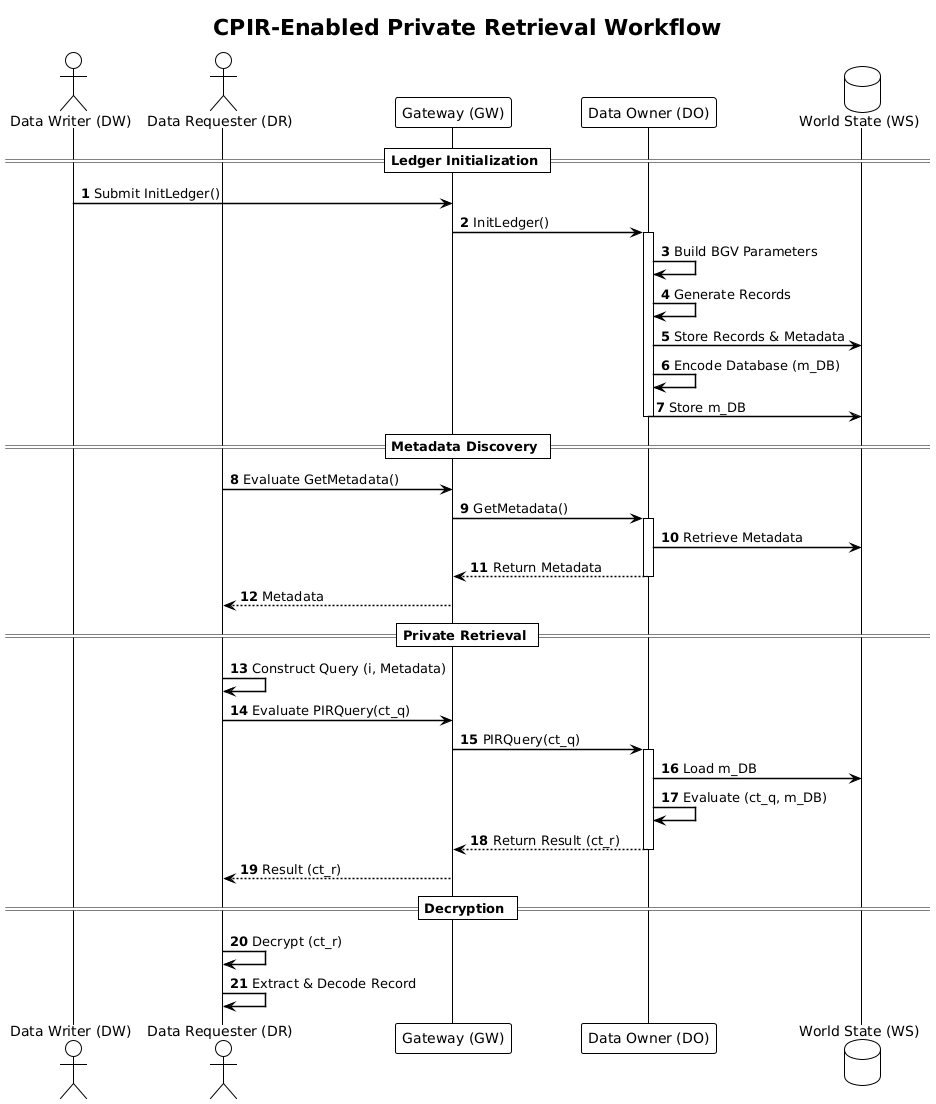
\includegraphics[width=\columnwidth]{1_workflow.png}
    \caption{Workflow. $\mathcal{DW}$ initializes the ledger via $\mathcal{GW}$, which triggers chaincode on endorsing
    peers ($\mathcal{DO}$). $\mathcal{DO}$ executes the protocol and persists state in world state ($m_{DB}$, metadata,
    JSON records). $\mathcal{DR}$ later obtains metadata, submits
    $ct_q=\emph{Enc}_{pk}(\encS{v_i})$, and $\mathcal{DO}$ evaluates
    $ct_r=\emph{Eval}(ct_q,m_{DB})$. The requester decrypts and slot-decodes the
    masked response, then extracts $J_i$ to reconstruct $d_i$.}
    \label{fig:system-overview}
\end{figure}

\subsection{POLYNOMIAL DATABASE CONSTRUCTION}
To enable PIR queries over structured ledger data, we must embed records into a plaintext polynomial \emph{$m_{DB}$} suitable 
for BGV evaluation. Our prototype adopts a fixed-width packing strategy, which proceeds in four steps.

\textbf{Step 1: Serialize to Byte Array.}
Each structured record $d_i$ is deterministically serialized to UTF-8 JSON
bytes. Every byte value in $[0,255]$ is embedded as one logical plaintext slot
in $\mathbb{Z}_T$. The evaluated implementation uses the batching-compatible
plaintext modulus $T=65537$; $T$ is not the byte alphabet size.

\textbf{Step 2: Calculate Slot Window.}
The implementation stores one serialized byte per logical slot. If $record_b$
is the maximum serialized record length in bytes, the fixed allocation is
rounded to the next multiple of eight:
\begin{equation}
\label{eq:record_s}
record_s=8\cdot\left\lceil\frac{record_b}{8}\right\rceil.
\end{equation}
For example, $record_b=126$ bytes gives $record_s=128$ logical slots.

\textbf{Step 3: Pack into Logical Slot Vector.}
Let $\dslots\in\mathbb{Z}_T^N$ be initialized to zero. Each serialized record
$d_i$ is assigned to its disjoint slot window
$J_i=\{i\cdot record_s,\dots,(i+1)\cdot record_s-1\}$:
\begin{equation}
\label{eq:packing}
\dslots[J_i[k]]=
\begin{cases}
\textsf{byte}(d_i[k]) & \text{if } k<|d_i|,\\
0 & \text{otherwise},
\end{cases}
\end{equation}
for $i\in[n]$ and $k\in[0,record_s-1]$. These entries are logical BGV slot
values supplied to the batching encoder, not the monomial-basis coefficients
of the resulting plaintext polynomial.

\textbf{Step 4: Batch-Encode the Database.}
The logical slot vector is mapped to a BGV plaintext by the batching encoder:
\begin{equation}
\label{eq:polynomial_db}
m_{DB}=\encS{\dslots}\in R_T.
\end{equation}
Internally, $m_{DB}$ is a polynomial in
$R_T=\mathbb{Z}_T[X]/(X^N+1)$, but its monomial coefficients are produced by
the batching transform and are not generally equal to the entries of
$\dslots$. This distinction allows polynomial multiplication inside $R_T$ to
decode as componentwise multiplication of logical slots.

\subsection{FEASIBILITY CONSTRAINTS}

\begin{figure*}[!htbp]
    \centering
    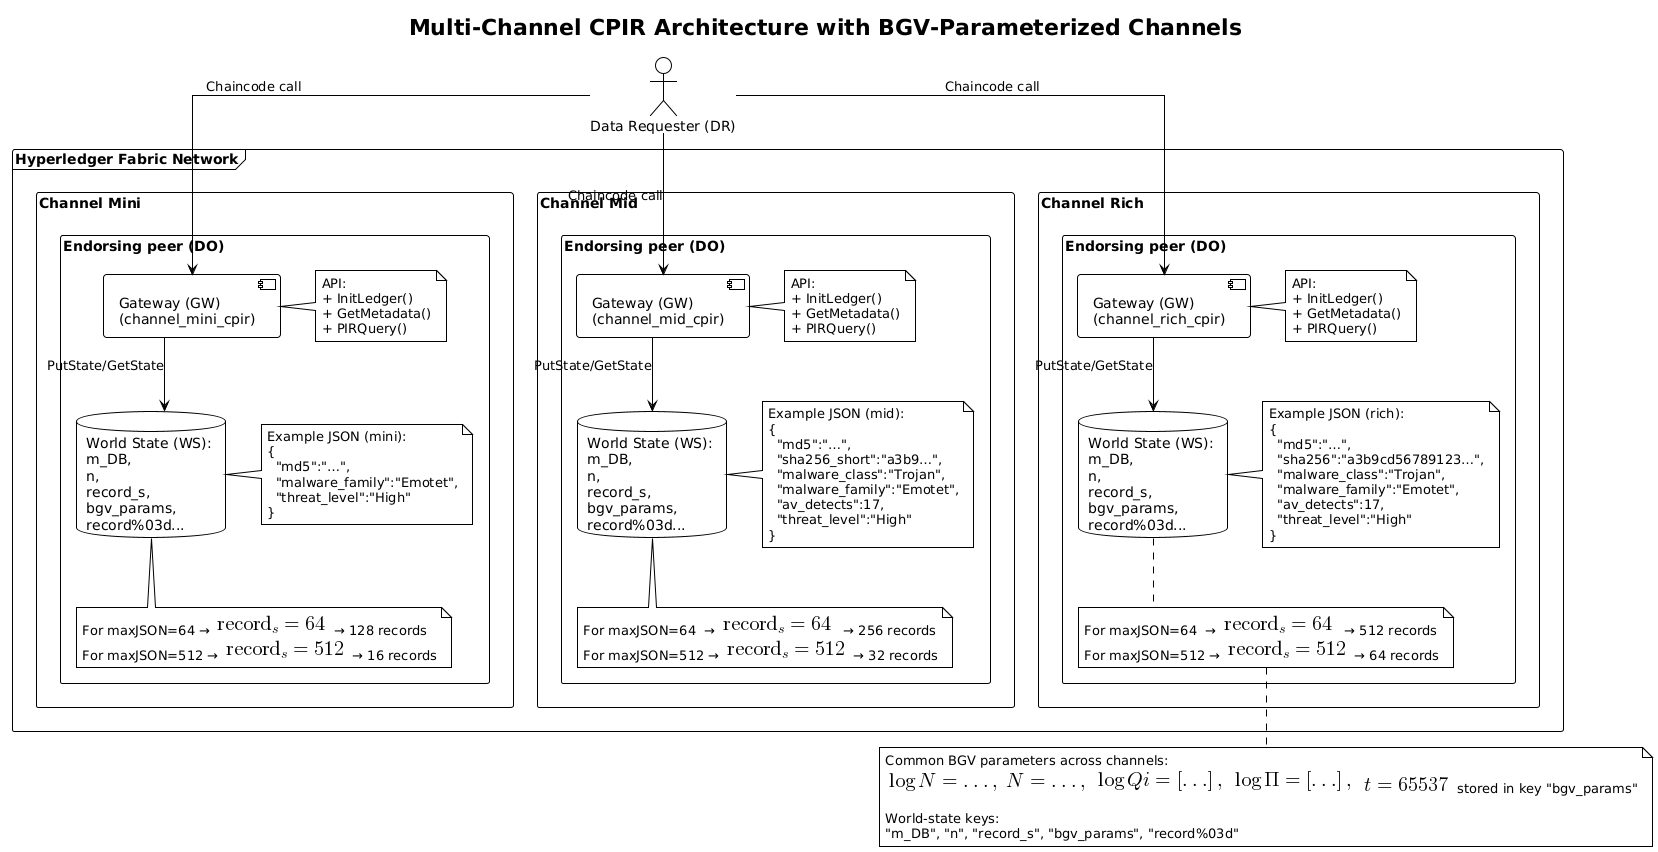
\includegraphics[width=\textwidth]{4_multi_channel_arc.png}
    \caption{Multi-channel CPIR architecture. 
    Each channel instantiates a separate CPIR chaincode and maintains its own \emph{$m_{DB}$} polynomial, 
    parameterized by $\log N$. This allows compact, mid-size, and rich CTI records to coexist under the same Fabric network.}
    \label{fig:multi-channel}
  \end{figure*}

Embedding records into the plaintext polynomial \emph{$m_{DB}$} is feasible only for parameter triples 
$(\log N, n, record_s)$ that satisfy \emph{all} of the following constraints.\footnote{The complete slot-packing 
workflow and parameter feasibility plots are given in the Supplementary Material (Figs.~S1–S2).}

\textbf{Constraint 1: Ring capacity.}
The total number of occupied slots cannot exceed the ring size:
\begin{equation}
    \label{eq:ring_capacity}
    n \cdot record_s \leq N.
\end{equation}
This represents the fundamental mathematical limit imposed by the cryptographic parameters. 
For example, with $\log N = 13$ ($N = 8192$) and $record_s = 224$, 
at most $\lfloor 8192/224 \rfloor = 36$ records can be packed.

\textbf{Constraint 2: Template-specific minima.}
We anticipate that different application scenarios require different record templates composed of distinct field combinations. 
Each template $\mu$ imposes a minimum slot requirement $record_{\mu,\log N}$, determined by its mandatory fields:

\begin{equation}
    \label{eq:template_minima}
    record_{\mu,\log N} = B_\mu + \sum_{i \in \mathcal{H}_\mu} |F_i| + O_\mu,
\end{equation}
where $B_\mu$ is the base structure size for template $\mu$,
$\mathcal{H}_\mu \subseteq {F_1, F_2, \dots, F_L}$, denotes the set of fields included in template $\mu$,
$|F_i|$ is the byte length of field $F_i$,
$O_\mu$ captures serialization overhead and metadata specific to template $\mu$.

\textbf{Constraint 3: Discrete allocation policy.}
Operationally, we restrict the slot window $record_s$ to a discrete set for implementation simplicity:
\begin{equation}
    \label{eq:discrete_allocation}
    record_s \in \mathcal{S},
    \mathcal{S} = \{64, 128, 224, 256, 384, 512\} \ \text{bytes}.
\end{equation}
This means that only certain fixed slot sizes are allowed,
simplifying client query construction and chaincode logic.

\noindent\textbf{Constraint hierarchy and feasibility.}
We summarize the three constraints as predicates:
\begin{subequations}
    \begin{align}
    \mathcal{C}(N,s,n) & : n \cdot s \leq N \quad, \\
    \mathcal{M}(\log N,s) & : s \geq record_{\mu,\log N} \quad, \\
    \mathcal{D}(s) & : s \in \mathcal{S} \quad.
    \end{align}
\end{subequations}
where $\mathcal{C}$ captures ring capacity, $\mathcal{M}$ captures template minima,
and $\mathcal{D}$ captures discrete allocation, $s$ denotes $record_s$ here for brevity. 
The overall feasibility condition is:
\begin{equation}
    \label{eq:feasibility_condition}
    \mathcal{F} \iff
    \mathcal{C}(N,s,n)\ \wedge\ \mathcal{M}(\log N,s)\ \wedge\ \mathcal{D}(s)
\end{equation}

\subsection{MULTI-CHANNEL ARCHITECTURE}

The packing strategy and feasibility constraints highlight an important observation: 
no single homomorphic parameter set can efficiently support the full diversity of dynamic CTI records encountered in practice.
Compact records fit comfortably under smaller rings, while full JSON objects with long cryptographic hashes exceed the 
slot budget of these configurations. To balance scalability and expressiveness, we design a \emph{multi-channel architecture} in 
Hyperledger Fabric, where each channel is provisioned with a distinct BGV parameter set and record template.

\textbf{a) Channel Mini} ($N=2^{13}$).  
Supports compact records with maximum scalability and lowest query latency. 
For example, with $N=8192$ slots, the system accommodates up to 128 records when $\max_i |d_i| \leq 64$ bytes, 
and 16 records when $\max_i |d_i| \leq 512$ bytes.

\textbf{b) Channel Mid} ($N=2^{14}$).
Targets medium-sized records that include MD5 and truncated SHA-256 fields alongside classification metadata. 
With $N=16384$ slots, the system supports up to 256 records at $\leq 64$ bytes or 32 records at $\leq 512$ bytes.

\textbf{c) Channel Rich} ($N=2^{15}$).
Handles the most detailed records, including full-length hashes and multiple metadata fields. 
Here, $N=32768$ slots allow up to 512 records at $\leq 64$ bytes or 64 records at $\leq 512$ bytes.

\noindent\textbf{Channel semantics.}  
As shown in Fig.~\ref{fig:multi-channel}, each channel maintains its own PIR chaincode instance and world state. 
The world state contains:
\begin{itemize}
    \item The \emph{polynomial view}: the packed plaintext polynomial \emph{$m_{DB}$} under key \emph{``m\_DB"}.
    \item The \emph{normal view}: JSON records stored optionally under keys \emph{``record\%03d"} for auditability.
    \item \emph{Metadata}: \emph{``n''}, \emph{``record\_s"} and \emph{``bgv\_params"}.
\end{itemize}

\subsection{WORKFLOW DETAILS}
The proposed system has five main routines, corresponding to 3 chaincode-side functions 
(\texttt{InitLedger}, \texttt{GetMetadata}, \texttt{PIRQuery}) and 2 client-side utilities (\texttt{FormSelectionVector}, 
\texttt{DecryptResult}). The detailed pseudocode for these routines is provided in the Supplementary Material (Algorithms~S1–S5).
Figure~\ref{fig:system-overview} provides the high-level overview. 
A Data Writer ($\mathcal{DW}$) provisions the database $D=\{d_0,\dots,d_{n-1}\}$, 
a Data Owner ($\mathcal{DO}$) maintains the polynomial \emph{$m_{DB}$} in world state and executes PIR evaluations, 
and a Data Requester ($\mathcal{DR}$) retrieves $d_i$ privately using homomorphic encryption.
The detailed steps are as follows:
\begin{enumerate}
    \item \textbf{$\mathcal{DW}$ submits initialization.}  
    $\mathcal{DW}$ calls \texttt{InitLedger} (Alg.~S1) via $\mathcal{GW}$ (\emph{submit}) 
    with inputs $(n,\,record_{s}^{\mathcal{DW}})$ and an optional hint $(\log N,\log Q_i,\log P_i,T)$. 
    Here $record_{s}^{\mathcal{DW}}$ denotes the maximum JSON size anticipated by the writer. 

    \item \textbf{$\mathcal{DO}$ validates and derives parameters.}  
    $\mathcal{DO}$ rounds the writer’s input to a discrete slot size 
    $record_{s}^{\mathcal{GW}} = 8 \cdot \lceil record_{s}^{\mathcal{DW}} / 8 \rceil$. 
    If $\log N$ is absent, the smallest feasible $\log N$ is chosen such that 
    $\mathcal{C}(N,record_{s}^{\mathcal{GW}},n)$ holds. 
    BGV parameters $\{\log N,N,\log Q_i,\log P_i,T\}$ are constructed and stored.

    \item \textbf{$\mathcal{DO}$ prepares records.}  
    Records $D=\{d_0,\dots,d_{n-1}\}$ are ingested or synthesized with $|d_i|\le record_{s}^{\mathcal{DW}}$. 
    The definitive slot allocation is then fixed as 
    $record_s = 8 \cdot \lceil \max_i |d_i| / 8 \rceil$ (discrete policy), 
    checked against feasibility predicates 
    $\mathcal{M}(\log N,record_s)$, $\mathcal{D}(record_s)$, $\mathcal{C}(N,record_s,n)$. 

    \item \textbf{Pack and persist.}  
    Each $d_i$ is serialized into the disjoint window
    $J_i=\{i\cdot record_s,\dots,(i+1)record_s-1\}$ of $\dslots$; unused
    slots are zero padded. Chaincode computes $m_{DB}=\encS{\dslots}$ at the
    maximum level and stores \emph{``m\_DB"}, \emph{``n"},
    \emph{``record\_s"}, and \emph{``bgv\_params"}, plus optional
    \emph{``record\%03d"} entries.
    
    \item \textbf{$\mathcal{DR}$ discovers metadata.}  
    $\mathcal{DR}$ calls \texttt{GetMetadata} (Alg.~S2) via \emph{evaluate} 
    to obtain $(n,record_s,\log N,N,T,\log Q_i,\log P_i)$. 
    This enables reconstruction of the cryptographic context. 

    \item \textbf{$\mathcal{DR}$ instantiates crypto context.}  
    From metadata, $\mathcal{DR}$ builds parameters, executes $\emph{KeyGen}(\lambda)\!\to\!(pk,sk)$, 
    and prepares encoder/encryptor objects. 

    \item \textbf{Form and encrypt query.}  
    For index $i\in[n]$, $\mathcal{DR}$ runs \texttt{FormSelectionVector}
    (Alg.~S3), sets $v_i[j]=1$ exactly for $j\in J_i$, computes
    $m_q=\encS{v_i}$, encrypts $ct_q=\emph{Enc}_{pk}(m_q)$, and serializes the
    ciphertext with Base64 encoding.

    \item \textbf{PIR query evaluation.}  
    $\mathcal{DR}$ issues \texttt{PIRQuery}($ct_q^{B64}$) (Alg.~S4) via
    \emph{evaluate}. $\mathcal{DO}$ reloads $m_{DB}$ if necessary and computes
    the single ciphertext--plaintext product
    $ct_r=\emph{Eval}(ct_q,m_{DB})$.

    \item \textbf{Decryption and reconstruction.}  
    $\mathcal{DR}$ runs \texttt{DecryptResult} (Alg.~S5), decrypts and
    slot-decodes the response to $u=v_i\odot\dslots$, extracts $u[J_i]$, removes
    zero padding, and reconstructs $d_i$.

\end{enumerate}

\noindent\textit{Remark (Single-record and multi-window selectors).}
The current protocol retrieves one logical record per query. Its slot-level
selector nevertheless contains $record_s$ consecutive ones because one record
spans an entire window; this is an expanded one-hot selector, not a multi-record
query. A future multi-record query could set ones on several disjoint windows
within the same length-$N$ selector. For fixed BGV parameters, ciphertext degree,
and level, that change does not enlarge the single ciphertext or add another HE
multiplication; it increases the useful selected payload and the client-side
extraction work. Designs using additional ciphertexts or larger parameters would
have different costs.

\section{SECURITY ANALYSIS}\label{sec:security}
We now demonstrate how our construction satisfies the security objective defined in Section~\ref{sec:proposed_system}B 
by reduction to the IND-CPA~\cite{noauthor_ciphertext_2025} security of the BGV scheme~\cite{cryptoeprint:2011/277} 
(implemented via Lattigo~\cite{noauthor_lattigo_2024}) under the RLWE assumption~\cite{peikert_lattice_2014}. 
Our system implements a single-server, single-round HE-based PIR construction by tailoring
Lattigo's PIR example~\cite{noauthor_lattigoexamples_nodate} into a non-threshold, 
windowed-slot variant designed for the Hyperledger Fabric chaincode environment.
This construction relies on the security guarantees of BGV and RLWE, which we leverage in our proof below.

\emph{Proof.}
For each record index $i\in[n]$, let $v_i=\mathbf{1}_{J_i}$ be the logical
slot-level window selector and let $m_{q,i}=\encS{v_i}\in R_T$ be its batched
plaintext encoding. The query is a randomized BGV encryption
$ct_{q,i}\leftarrow\emph{Enc}_{pk}(m_{q,i})$. The selector entries are defined
in logical slot order before encoding; they are not asserted to be the
monomial-basis coefficients of $m_{q,i}$.

\emph{Indistinguishability Game.}
An honest-but-curious peer adversary $\mathcal{A}$ chooses two record indices
$i_0,i_1\in[n]$. The challenger samples $b\leftarrow\{0,1\}$, forms
$m_{q,b}=\encS{v_{i_b}}$, and returns
\[
ct_q\leftarrow\emph{Enc}_{pk}(m_{q,b}),\qquad
ct_r=\emph{Eval}(ct_q,m_{DB}).
\]
The adversarial view is
$View_{\mathcal{A}}=\{ct_q,ct_r,m_{DB},pp,\mathcal{L}\}$, where the public
parameters, encoded plaintext database, and allowed leakage are independent of
$b$. By IND-CPA security, encryptions of $m_{q,0}$ and $m_{q,1}$ are
computationally indistinguishable. Moreover,
$ct_r=\emph{Eval}(ct_q,m_{DB})$ is deterministic public post-processing of the
challenge ciphertext with fixed $m_{DB}$. Therefore the pair
$(ct_q,ct_r)$ remains computationally indistinguishable between the two games.
Any non-negligible distinguisher for the complete view yields an IND-CPA
distinguisher by applying the same public evaluation to its challenge
ciphertext. Hence\footnote{See App.~6 in~\cite{mahdavi_inspire_2025} and
Cor.~2 in~\cite{simplepir_2023} for similar \emph{formal} proofs.}
\[
\left|\Pr[b'=b]-\tfrac{1}{2}\right|\leq\operatorname{negl}(\lambda).
\]

\emph{Corollary 1 (Single Read Index Privacy).}
For one query, an adversary without $sk$ cannot distinguish which of two
allowed record windows was encoded in $ct_q$ except through $\mathcal{L}$.
This claim protects the request index; it does not assert confidentiality of
the plaintext database from the data-owning peer, which stores $m_{DB}$ and may
also store the corresponding JSON records.

\emph{Corollary 2 (Repeated Reads).}
Fresh randomized encryptions of any two equal-length sequences of encoded
selectors are computationally indistinguishable by a standard hybrid argument,
subject to the leakage $\mathcal{L}$. For each round, evaluation applies the
same fixed-parameter ciphertext--plaintext multiplication to the full encoded
ring representation, independently of which logical window $J_i$ contains
ones. The evaluator performs no data-dependent rotation, reduction, or early
termination that would reveal the selected window.

\section{PERFORMANCE EVALUATION}\label{sec:evaluation}
\subsection{EXPERIMENTAL SETUP}

All experiments were executed on a local Ubuntu~24.04 host running under WSL2 on an Intel~Core~i5-3380M~CPU 
(2~cores/4~threads, 2.90~GHz) with 7.7~GB of RAM and a 1~TB~SSD. 
During evaluation, the average available memory was 6.9~GB with a 2~GB swap partition, 
and the root filesystem reported 946~GB of free space.
The software stack consisted of Go~1.24.1, Docker~27.4.0, and Docker~Compose~v2.31.0, 
hosting Hyperledger~Fabric~v2.5 with LevelDB as the world-state database and a Solo ordering service, using recommended settings 
(\emph{BatchSize.AbsoluteMaxBytes}=99~MB, \emph{PreferredMaxBytes}=2~MB per block).
The network configuration comprised a single organization with one peer per channel, 
sufficient for privacy evaluation, though it can be extended to multiple peers and organizations as needed.

Our implementation employs Fabric~GO~SDK~\cite{fabric_gateway_pkg_client_nodate} for blockchain interactions and
the \emph{Lattigo}~v6 library~\cite{noauthor_lattigo_2024} as the homomorphic encryption backend.
Lattigo provides a Go-native implementation of the BGV scheme~\cite{cryptoeprint:2011/277},
whose security and correctness have been validated in prior literature. 
Accordingly, our focus is on evaluating its \emph{practical performance within a permissioned blockchain environment} for 
enabling \emph{private reads} from world state, rather than re-verifying the theoretical properties of BGV itself.

Unless otherwise stated, each reported value represents the mean of 20~executions under both cold and warm cache conditions, 
cross-verified against peer logs for consistency.

\subsection{CRYPTOGRAPHIC PERFORMANCE}

\noindent\textbf{Parameter Configuration.}
Table~\ref{tab:params} summarizes the BGV parameter sets used in our evaluation, 
including the ring dimension $N$, ciphertext modulus chain $(\log Q_i, \log P_i)$, 
plaintext modulus $T$, slot allocation $record_s$, and database size $n$. 
Each configuration corresponds to one Fabric channel and maintains a feasible 
packing ratio as defined in Section~\ref{sec:proposed_system}.

\begin{table}[!htbp]
\caption{Default BGV Parameter Configuration per Channel}
\label{tab:params}
\centering
\begin{tabular}{|c|c|c|c|c|c|}
\hline
$N$ & $\log Q_i$ & $\log P_i$ & $T$ & $record_s$ & $n$  \\
\hline
$2^{13}$ & [54] & [54] & 65537 & 128 & 64 \\
$2^{14}$ & [54] & [54] & 65537 & 224 & 73 \\
$2^{15}$ & [54] & [54] & 65537 & 256 & 128 \\
\hline
\end{tabular}
\end{table}

\noindent\textbf{Overall Results.}
Table~\ref{tab:crypto-times} lists the measured execution time of core cryptographic operations 
(\emph{KeyGen}, \emph{Enc}, \emph{Eval}, and \emph{Dec}) for each evaluated ring dimension~$N$. 
\begin{table}[!htbp]
  \caption{Execution Time of Cryptographic Operations (ms)}
  \label{tab:crypto-times}
  \centering
  \begin{tabular}{|c|c|c|c|c|}
  \hline
  $N$ & \emph{KeyGen} & \emph{Enc} & \emph{Eval} & \emph{Dec} \\
  \hline
  $2^{13}$ & 27.7 & 11.7 & 16.9 & 5.1 \\
  $2^{14}$ & 42.7 & 27.7 & 30.7 & 11.9 \\
  $2^{15}$ & 55.0 & 49.8 & 64.8 & 15.6 \\
  \hline
  \end{tabular}
\end{table}

Figure~\ref{fig:latency-stages} consolidates the main cryptographic evaluation metrics:
(A)~end-to-end latency by algorithmic stage,
(B)~serialized artifact size, \footnote{Extended cryptographic object sizes and world-state footprints
are reported in Table~S1–S2 of the Supplementary Material.} and
(C)~slot utilization ratio within the packed database polynomial \emph{$m_{DB}$}.

\begin{figure}[!ht]
\centering
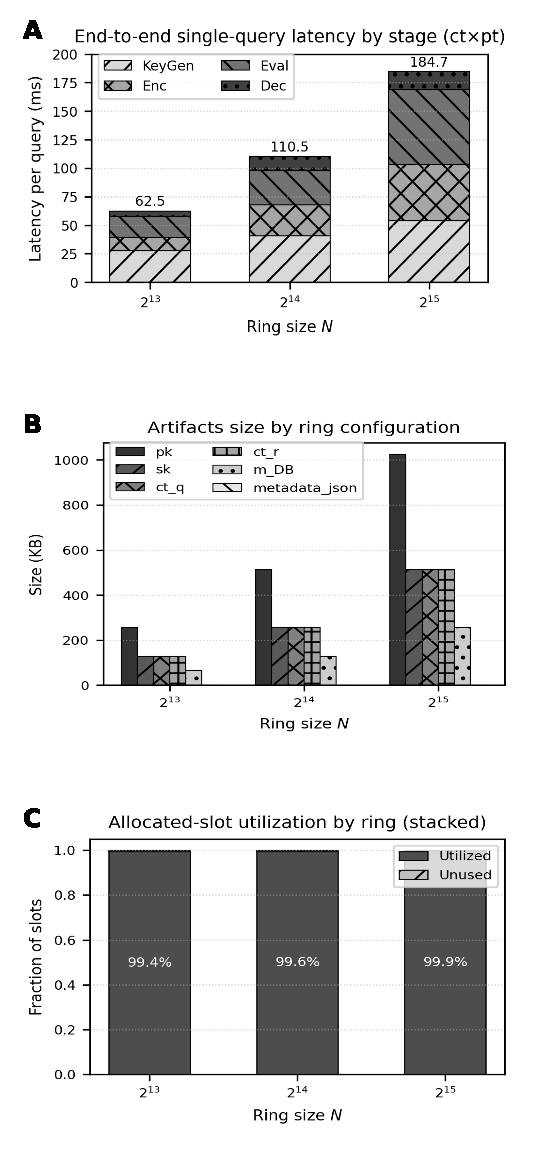
\includegraphics[width=\columnwidth]{plate_col.pdf}
\caption{Cryptographic performance of the BGV-based CPIR system: 
(A)~latency by algorithmic stage, (B)~artifact size by ring configuration, and 
(C)~allocated-slot utilization.}
\label{fig:latency-stages}
\end{figure}

\subsection{BLOCKCHAIN PERFORMANCE}

\noindent\textbf{Chaincode Execution Timings.} 
Figure~\ref{fig:chaincode-timings} visualizes the average server-side execution time of the main chaincode functions across three channels, 
each corresponding to a different ring size $N$.

\begin{figure}[!htbp]
    \centering 
    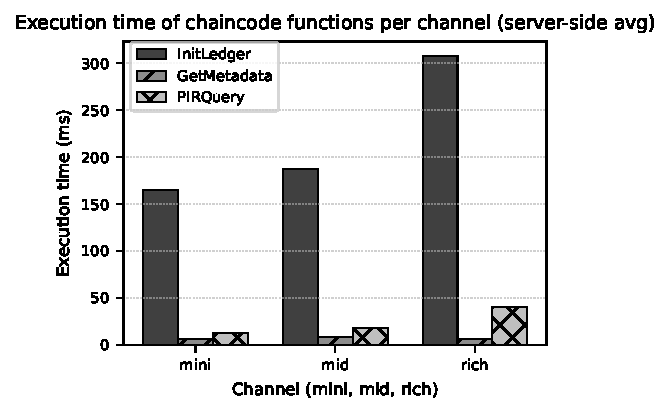
\includegraphics[width=\columnwidth]{chaincode_timings_bw.pdf} 
    \caption{Average chaincode execution time by function and ring size. Each bar represents the 
    mean execution time over multiple epochs.} \label{fig:chaincode-timings} 
\end{figure}

\noindent\textit{Remark (execution paths).}  
Transactions that modify world state (e.g., \texttt{InitLedger}) are issued via the 
\emph{submit} path and committed through Solo ordering,
while read-only operations (\texttt{GetMetadata}, \texttt{PIRQuery}) use the 
\emph{evaluate} path, bypassing block creation and ordering.  

\noindent\textbf{Blockchain Performance.} 
On-chain network behavior is reported in Table~\ref{tab:pirquery-netio}, which presents the average peer-side 
network I/O per \texttt{PIRQuery} transaction across the three channel configurations\footnote{For visual blockchain-side evaluation of the 
system across three channels, please refer to Figure~S3 in the Supplementary Material.}.

\begin{table}[!htbp]
  \centering
  \caption{Peer network I/O per PIRQuery (avg, KB/tx)}
  \label{tab:pirquery-netio}
  \begin{tabular}{|c|c|c|}
  \hline
  Channel & $N$ & NET I/O (KB/tx) \\
  \hline
  mini  & $2^{13}$ & 524.62 \\
  mid   & $2^{14}$ & 1042.09 \\
  rich  & $2^{15}$ & 2072.88 \\
  \hline
  \end{tabular}
\end{table}

\subsection{OVERALL SYSTEM PERFORMANCE}
  
\noindent\textbf{End-to-End Workflow Summary.}
Based on the data in Table \ref{tab:crypto-times} and Figure \ref{fig:chaincode-timings},
we now to summarize two main operational workflows in the system, involving $\mathcal{DW}$ and $\mathcal{DR}$, 
while $\mathcal{DO}$ is implicitly involved as the executing peer during private queries.

The first workflow corresponds to $\mathcal{DW}$ initializing the ledger through \texttt{InitLedger}, 
which packs and encodes the plaintext database \emph{$m_{DB}$} into world state. 

The second workflow corresponds to $\mathcal{DR}$ performing a private query by sequentially 
executing \texttt{GetMetadata} → \emph{KeyGen} → \emph{Enc} → \texttt{PIRQuery} → \emph{Dec}.
The PIR evaluation itself is performed by $\mathcal{DO}$ (endorsing peer) using ciphertext--plaintext 
multiplication during the evaluate transaction.

Table~\ref{tab:end2end} summarizes the cryptographic and blockchain timings for both workflows, 
averaged across all three channel configurations.

\begin{table}[!htbp]
    \caption{End-to-End Performance Analysis (ms)}
    \label{tab:end2end}
    \centering
    \begin{tabular}{|c|c|c|c|}
    \hline
    {Workflow} & 
    \shortstack{{Cryptographic} \\ {Operations (ms)}} & 
    \shortstack{{Blockchain} \\ {Operations (ms)}} & 
    \shortstack{{Total Time} \\ {(ms)}} \\
    \hline
    $\mathcal{DW}$'s Upload  & 0.0 & 220.0 & 220.0 \\
    $\mathcal{DR}$'s Query  & 82.4 & 30.5 & 112.9 \\
    \hline
    \end{tabular}
\end{table}

\begin{table*}[!htbp]
    \centering
    \caption{Comparison with existing privacy-preserving query systems}
    \label{tab:comparison-related}
        \begin{tabular}{|c|c|c|c|c|c|c|c|c|}
        \hline
        \textbf{Work} &  
        \shortstack{\textbf{Targeted} \\ \textbf{System}} &
        \shortstack{\textbf{Privacy} \\ \textbf{Technique}} &
        \shortstack{\textbf{Execution} \\ \textbf{Location}} &
        \shortstack{\textbf{Targeted} \\ \textbf{Operation}} &
        \shortstack{\textbf{Comm. Cost} / \\ \textbf{Query (MB)}} &
        \shortstack{\textbf{E2E Query} \\ \textbf{Time (ms)}} &
        \shortstack{\textbf{Db Size} / \\ \textbf{(\# of records)}} &
        \shortstack{\textbf{Record Size} / \\ \textbf{length (bytes)}} \\
        \hline
        \cite{kumar_debpir_2025} & HLF  & OT & on-chain & read / write & N/A & 600 & 10,000 & N/A \\
        \cite{kumar_bron_2024} & HLF & ZKP & on-chain & read / write & N/A & N/A & 10,000 & N/A \\
        \cite{xiao_cloak_2024} & Blockchain  & DPF & off-chain & read & 0.0002-0.0005 & 0.4-0.5 & 4-64 & 16-32 \\
        \cite{mazmudar_peer2pir_2025} & IPFS & HE-PIR & off-chain & read & 10-15 & 500-16,000 & 1,000-1M & 256,000 \\
        \cite{Kaihua2019applying} & Bitcoin & Hybrid PIR & off-chain & read & 0.65 & 2840 & 7,688-512,460 & 62-876 \\
        \textbf{Ours} & \textbf{HLF} & \textbf{HE-PIR} & \textbf{on-chain} & \textbf{read} & \textbf{1-2} & \textbf{112.9} & \textbf{16-512} & \textbf{64-512} \\
        \hline
        \end{tabular}
\end{table*}

\noindent\textbf{Projected Cost for PIR Query.}
Among our results, for the ring size $2^{15}$ configuration, issuing 100/1000/10000 private queries incurs 
$\approx $207MB / 2.07 GB / 20.7 GB of peer-side network I/O with an associated chaincode evaluation time 
of $\approx$0.07/0.67/6.73 minutes, respectively, when using our protocol, as shown in Table \ref{tab:batch-cost-rich} 
and Figure \ref{fig:batch-cost-rich}.

\begin{table}[!htbp]
    \centering
    \caption{Projected cost for multiple PIR queries at $2^{15}$ (peer perspective)}
    \label{tab:batch-cost-rich}
    \begin{tabular}{|c|c|c|}
    \hline
    \# Transactions & Total Bandwidth (MB) & Total Time (min) \\
    \hline
    100   & 207.3  & 0.07 \\
    1000  & 2073.0 & 0.67 \\
    10000 & 20730.0 & 6.73 \\
    \hline
    \end{tabular}
\end{table}

\begin{figure}[!htbp] 
    \centering 
    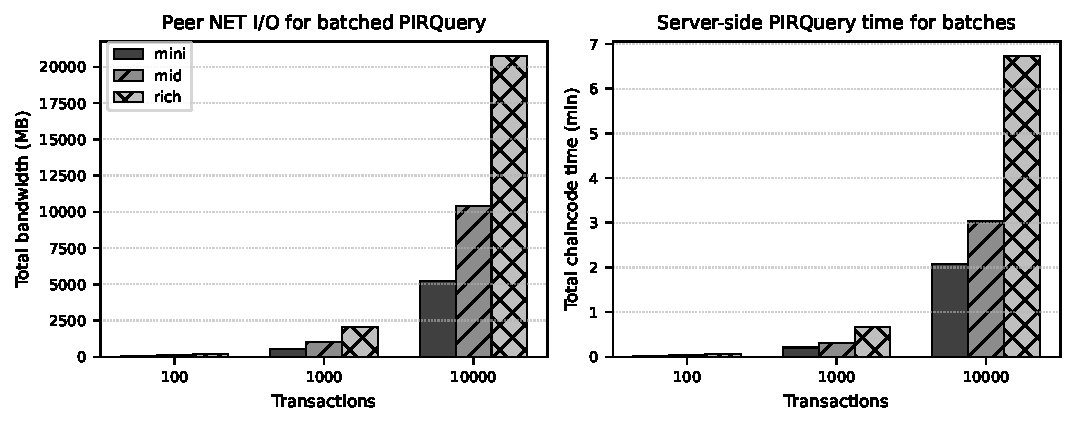
\includegraphics[width=\columnwidth]{pirquery_batch_cost_bw.pdf} 
    \caption{Projected cost for multiple PIR queries at $2^{15}$ (peer perspective)} 
    \label{fig:batch-cost-rich} 
\end{figure}

\noindent\textit{Remark (on network I/O measurement).} 
The network I/O values in Table~\ref{tab:pirquery-netio} and Table~\ref{tab:batch-cost-rich} were obtained from \emph{docker stats} 
snapshots collected for the \emph{peer0.org1.example.com} and \emph{orderer0.group1.orderer.example.com} containers during each benchmark epoch. 

\section{DISCUSSION}\label{sec:discussion}

\subsection{FUTURE WORK AND OUTLOOK}
Although our prototype validates this concept, several challenges remain in performance, scalability, and deployment.
Future research should address \emph{(i)} side-channel resilience through constant-time chaincode evaluation and standardized 
ciphertext serialization to mitigate timing and size-based leakages. 
\emph{(ii)} Scaling beyond moderate database sizes will require some form of sublinear or sharded CPIR, 
similar to~\cite{simplepir_2023,piano_pir_2024,hintless_pir_2024,ypir_2024}, yet adapted to Fabric’s architecture and resource constraints.
Moreover, \emph{(iii)} extending the current ciphertext–plaintext (\emph{ct}×\emph{pt}) evaluation to fully encrypted-database (\emph{ct}×\emph{ct}) 
computation would enable richer on-chain analytics under encryption, though it demands relinearization, rotation, and modulus-switching 
capabilities within Fabric’s resource limits. 
\emph{(iv)} Dynamic ledger updates, (\texttt{addRecord}) operation would allow incremental growth without full reinitialization,
raising questions around re-encoding and key management. 
\emph{(v)} Selective field-level retrieval through adaptive packing could enable varying length records and partial access control.
\emph{(vii)} Deployment optimization is crucial. In our setup, the chaincode ran in \emph{development mode} as an external service, 
causing duplicated gRPC transmissions for each ciphertext (\emph{ct\textsubscript{q}}, \emph{ct\textsubscript{r}}) due to two network 
hops—client$\leftrightarrow$peer and peer$\leftrightarrow$chaincode. This resulted in $\approx$2072~KB per query for $N=2^{15}$, 
as shown in Table~\ref{tab:batch-cost-rich}. Running the chaincode \emph{in-process} within the peer would eliminate the second hop, 
halving the network cost to $\approx$1024~KB per query.

\subsection{RELATED WORK COMPARISON}

Table~\ref{tab:comparison-related} contrasts our proposed PIR-based \emph{private reads} mechanism with several recent works 
discussed in Section~\ref{sec:introduction},
that integrate Private Information Retrieval (PIR) or related cryptographic mechanisms 
to achieve query privacy across different domains.
The comparison focuses on six key aspects:
\emph{(i)} which target system the privacy solution is built for,
\emph{(ii)} the underlying privacy primitive (CPIR, IT-PIR, hybrid, DPF etc),
\emph{(iii)} whether privacy computation occurs on-chain (via smart contracts or chaincode) or off-chain,
\emph{(iv)} the targeted operation (read-only or read/write),
\emph{(v)} communication cost per query (in MB),
\emph{(vi)} end-to-end query time (in ms),
\emph{(vii)} database size (number of records), and
\emph{(viii)} record size (in bytes).

\section{CONCLUSION}\label{sec:conclusion}
This paper presented a Private Information Retrieval (PIR) mechanism for enabling \emph{private reads} in Hyperledger~Fabric, 
allowing endorsing peers to evaluate encrypted queries without learning which record was accessed. 
The proposed chaincode performs ciphertext–plaintext (\emph{ct×pt}) homomorphic multiplication directly within 
\emph{evaluate} transactions, preserving Fabric’s endorsement and audit semantics. 
Our prototype achieves an average end-to-end latency of 113~ms and a peer-side execution time below 42~ms, 
with approximately 2~MB of peer network traffic per query in development mode—reducible to about 1~MB under in-process deployment. 
Storage profiling shows near-linear growth in both block and world-state sizes as the ring dimension scales, 
and parameter analysis confirms practical support for up to 512~records of 64~bytes each under $2^{15}$.  
These results validate the feasibility of PIR-based \emph{private reads} in permissioned ledgers, 
offering millisecond-scale query latency and full compatibility with Fabric’s architecture. 

\bibliographystyle{IEEEtran}
\bibliography{bibliography}

\newpage

\begin{IEEEbiography}[{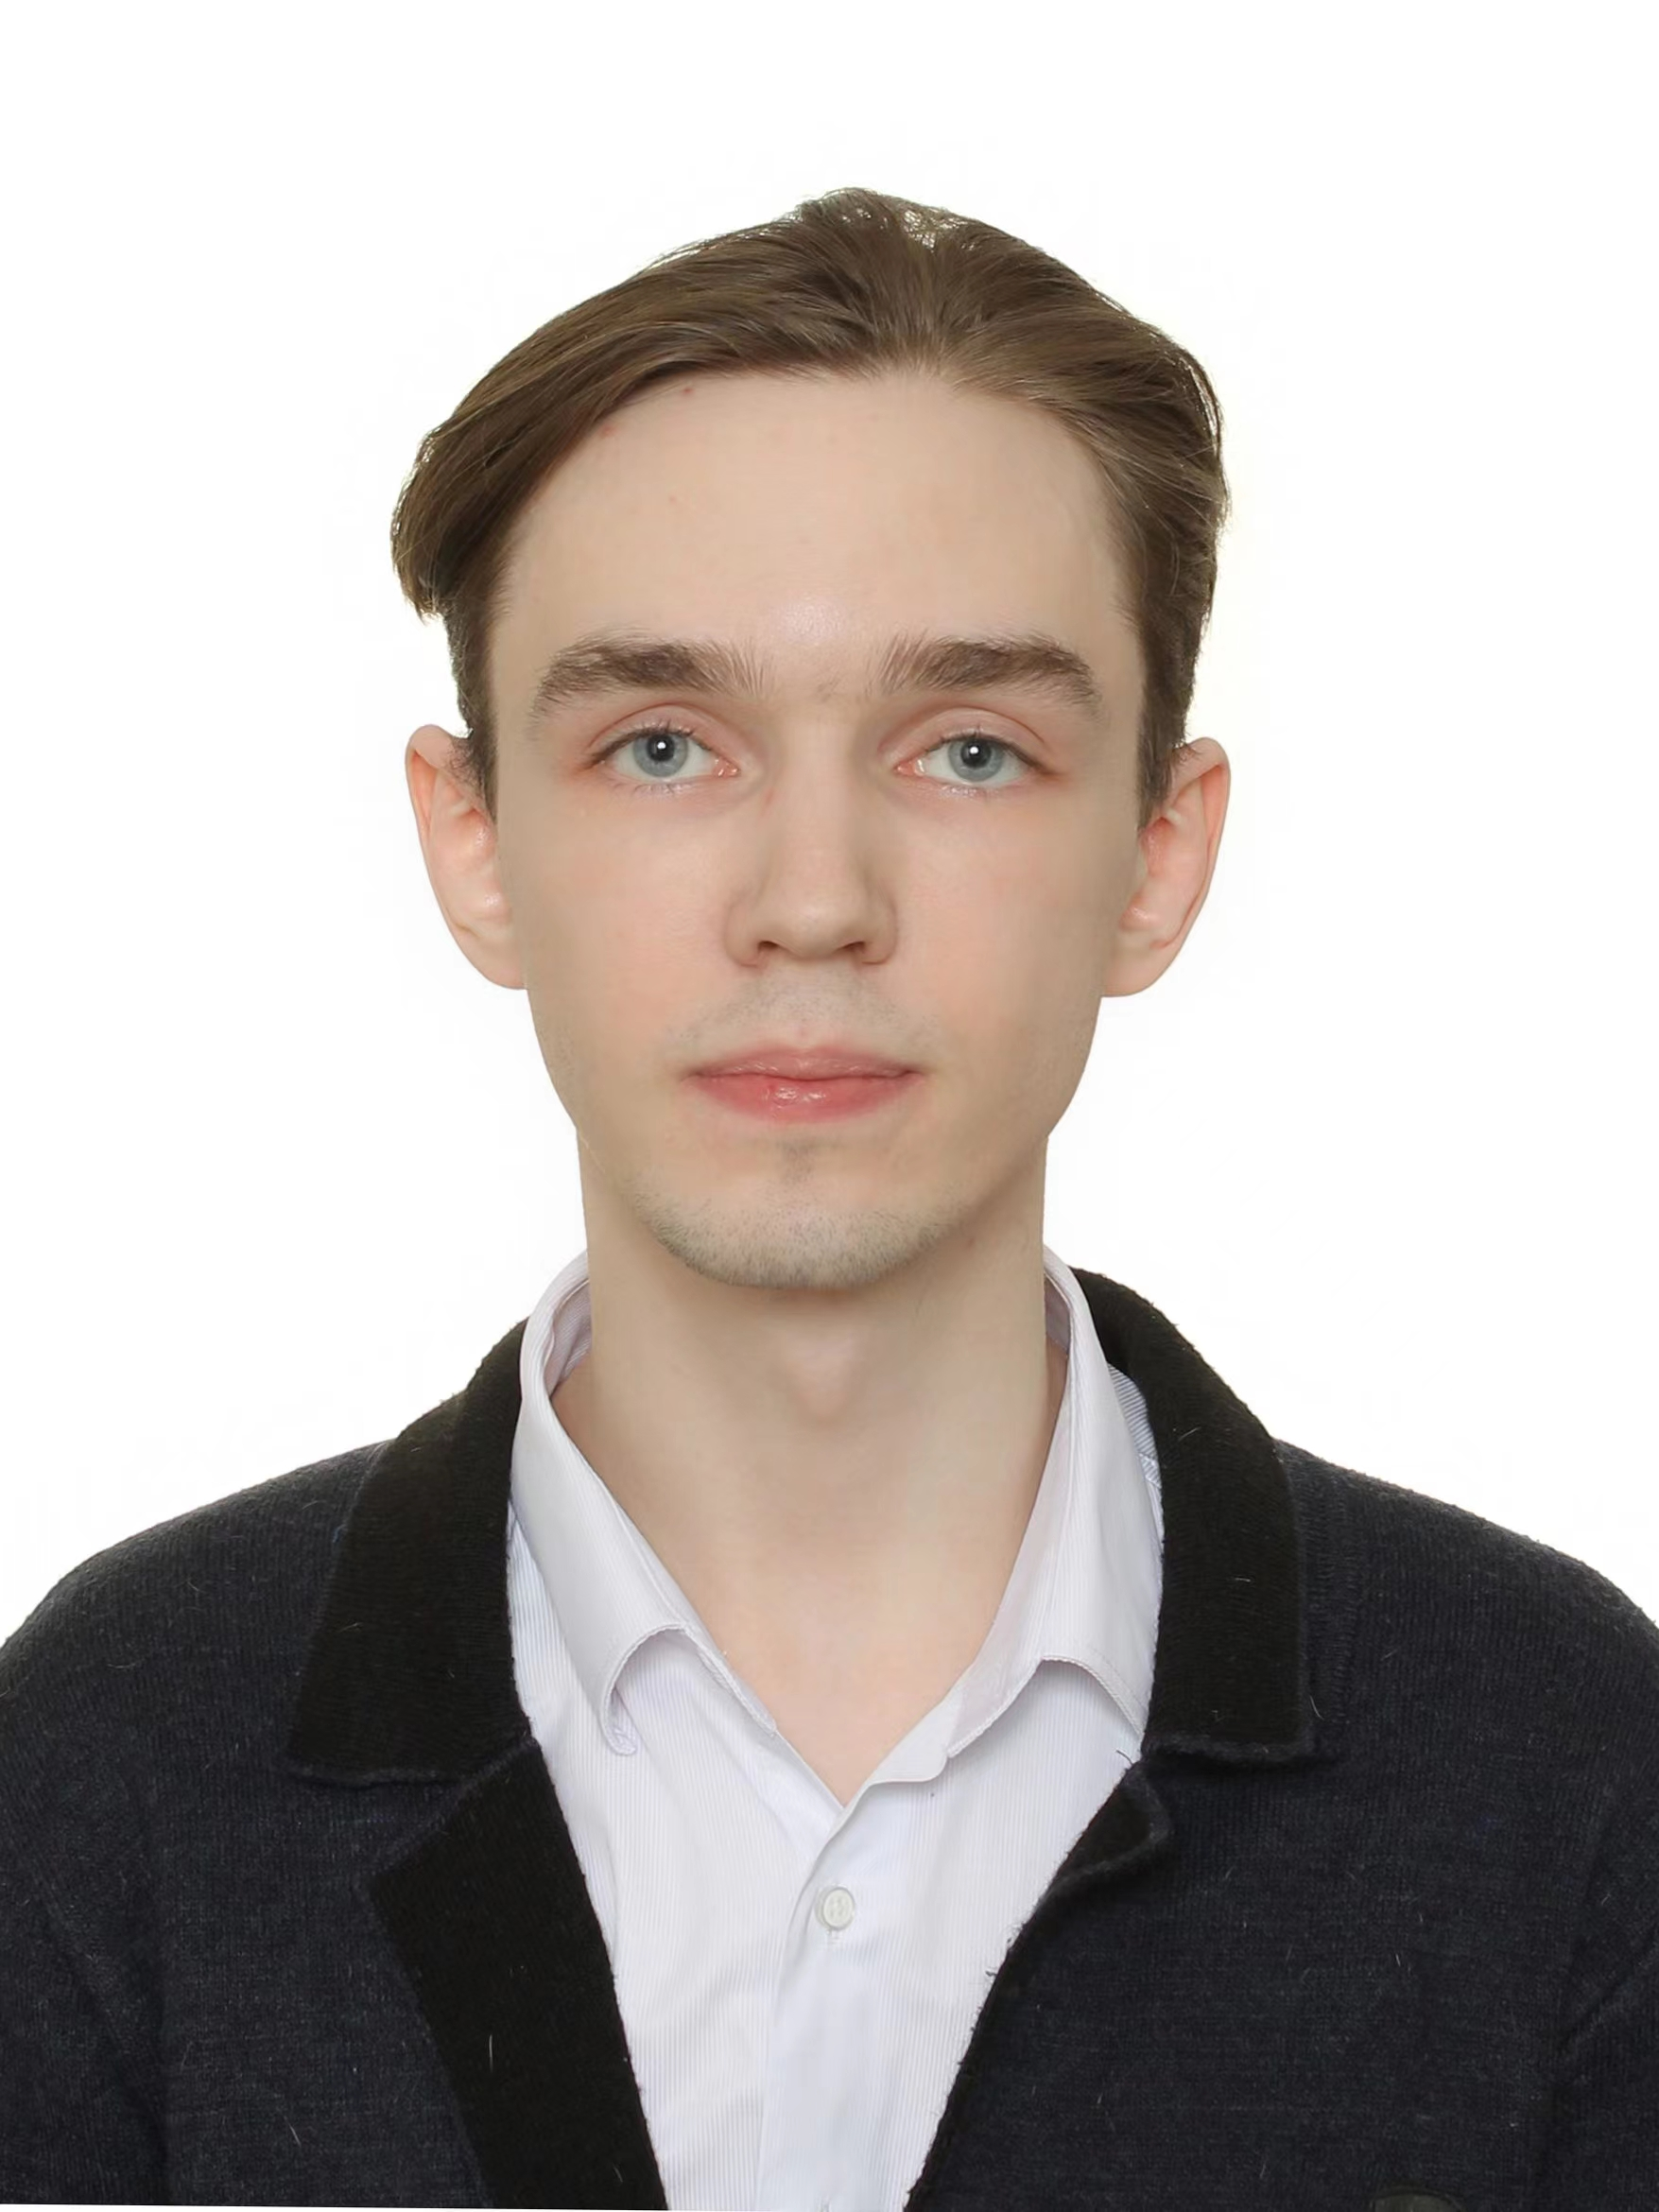
\includegraphics[width=1in,height=1.25in,clip,keepaspectratio]{arturiasenovets.jpg}}]{ARTUR IASENOVETS}
~is currently pursuing the M.S. degree in the School of Cybersecurity and Information Law at the Chongqing University of Posts and Telecommunications. 
His research interests include blockchain, privacy-enhancing technologies, and cyber threat intelligence.
\end{IEEEbiography}

\begin{IEEEbiography}[{
\includegraphics[width=1in,height=1.25in,clip,keepaspectratio]{feitang.png}}]{FEI TANG}
~received the Ph.D. degree in information security from the Institute of Information Engineering, 
Chinese Academy of Sciences, in 2015. He is currently a Professor with the Chongqing University of Posts and Telecommunications. 
His research interests include public-key cryptography, data security, and so on.
\end{IEEEbiography}

\begin{IEEEbiography}[{
\includegraphics[width=1in,height=1.25in,clip,keepaspectratio]{huihuizhu.jpg}}]{HUIHUI ZHU}
~is currently working toward a Ph.D. degree in the School of Computer Science and Technology, 
Chongqing University of Posts and Telecommunications, Chongqing, China. His recent research interests include secure multi-party 
computation and information security.
\end{IEEEbiography}

\begin{IEEEbiography}[{
\includegraphics[width=1in,height=1.25in,clip,keepaspectratio]{pingwang.jpg}}]{PING WANG}
~received her M.S. degree from Chongqing University of Posts and Telecommunications in 2022. She is currently pursuing a Ph.D. 
degree in the School of Computer Science and Technology at Chongqing University of Posts and Telecommunications. Her present research 
interest includes privacy-preserving computing.
\end{IEEEbiography}

\begin{IEEEbiography}[{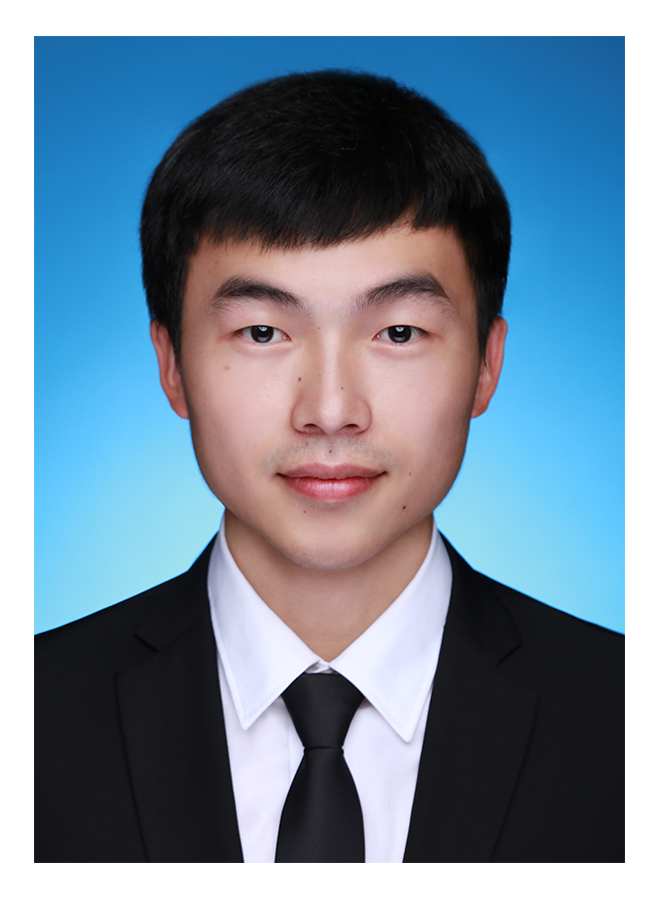
\includegraphics[width=1in,height=1.25in,clip,keepaspectratio]{leiliu.jpg}}]{LEI LIU}
~received his M.S. degree in Integrated Circuit Engineering from Fuzhou University in 2018. He is currently pursuing 
a Ph.D. degree in the School of Computer Science and Technology at Chongqing University of Posts and Telecommunications. 
His research interests include data security and blockchain.
\end{IEEEbiography}

\vfill\pagebreak

\end{document}
